\capitulo{5}{Aspectos relevantes del desarrollo del proyecto}

\section{Datasets}\label{datasets}

\hypertarget{gtzan-dataset}{%
\subsection{GTZAN Dataset}\label{gtzan-dataset}}

Las versiones iniciales del clasificador fueron desarrolladas sobre el
conjunto de datos para clasificación de música GTZAN.

Este conjunto de datos \cite{gtzan_paper} fue creado por George Tzanetakis en el año 2001 a
partir de pequeños fragmentos de 30s extraídos de CDs, DVDs, Casettes y
grabaciones de la radio. Es uno de los conjuntos de datos más utilizados
en los sistemas de reconocimiento de géneros musicales.

Este conjunto de datos está formado por 10 géneros, cada uno con 100
segmentos diferentes en formato .wav, mono, 16 bits de profundidad y una
frecuencia de muestreo de 22050HZ. Los géneros son: Blues, Classical, Country, Disco, Hip Hop, Jazz, Metal, Pop, Reggae y Rock.

Si bien este conjunto de datos es muy variado al contener 10 géneros muy diferentes entre sí y múltiples fuentes de audio, presenta varios problemas:

\begin{itemize}
\itemsep0em
\item
  \textbf{Etiquetas incorrectas}: Estos es debido a que la clasificación
  de música es una tarea complicada incluso para el ser humano, siendo
  la precisión media del 70\%, como explora \cite{cnn_vs_human_acc_music}.
\item
  \textbf{Distorsiones}: Si bien las distorsiones son una característica
  del conjunto de datos, es recomendable distorsionar la música mediante
  preprocesamiento, ya que no todos los casos de usuo requieren de un conjunto de 
  datos con distorsiones. Los problemas relacionados 
  con la calidad del conjunto de datos han sido explorados en \cite{gtzan_analysis}.
\item
  \textbf{Conjunto Reducido}: Únicamente disponemos de 100 segmentos de
  30s por etiqueta.
\item
  \textbf{Conjunto Obsoleto}: El conjunto fue creado a principios de los
  años 2000, por lo que no refleja los estilos de las dos últimas décadas de música.
\end{itemize}


\subsection{GTZAN Extended}\label{gtzan-extended}

Como alternativa al conjunto de datos GTZAN, se decidió crear una versión
extendida con 300 canciones por cada género. Este conjunto de datos fue
creado a partir de playlists de Spotify creadas por la comunidad o por la propia Spotify.

Para esta tarea se ha utilizado la herramienta \textbf{dataset-tools node}, introducida en el manual de programador, que permite descargar las previsualizaciones de canciones de 30s. Para seleccionar las playlists se ha usado el explorador de Spotify, y se han descargado playlists del género en concreto. 

Si bien este nuevo conjunto de datos extendido incluye 2000
canciones nuevas, fue creado a partir de las canciones más populares de
Spotify del siglo XX, por lo que no tenemos una variedad real de
canciones.

Este conjunto de datos extendido ha sido publicado en Kaggle \cite{GtzanExt16:online}.


\subsection{Ludwig Dataset}\label{ludwig-dataset} 

El Ludwig Dataset \cite{LudwigMu18:online} es un conjunto de datos de música creado
específicamente para este proyecto.

Existen una gran variedad de conjuntos de datos destinados al análisis
de música, pero no hay ninguno que cumpla con todos los requisitos del
proyecto.
\begin{itemize}

\itemsep0em
\item
  Géneros
\item
  Subgéneros
\item
  Estados de Ánimo
\item
  Ficheros de Audio
\item
  Canciones asociadas con Spotify
\item
  Etiquetas Supervisadas. 
\end{itemize}

Para poder crear este conjunto de datos, ha sido necesario cruzar tres
fuentes de datos distintas. El proceso de generación ha sido detallado mediante un diagrama en el anexo C (Diseño). 
\begin{itemize}
\itemsep0em
\item
  \textbf{Discogs}: Discogs \cite{a2022_discogs} es el Marketplace de música más importante del mundo, cada
  item está categorizado por género y subgéneros. Discogs dispone de una
  API pública que permite obtener datos sobre los distintos elementos.
\item
  \textbf{AcousticBrainz y MusicBrainz}: MusicBrainz \cite{musicbrainz} es una base de datos
  colaborativa de música, no es muy completa pero cada elemento tiene un
  MBID que es compartido con AcousticBrainz y Discogs.\\
  ~\\
  AcousticBrainz es un proyecto del Music Technology Group de la
  Universitat de Pompeu Fabra \cite{bogdanov2019acousticbrainz} que permite analizar y clasificar
  canciones a partir de la onda sonora.\\
  Este proyecto incluye una API pública en la que se pueden consultar detalles de
  canciones, como estados de ánimo o etiquetas obtenidas a partir de múltiples clasificadores. Se puede consultar los datos de una canción a partir de su MBID.
\item
  \textbf{Spotify}: La API pública de Spotify \cite{spotify_docs} dispone de un endpoint de búsqueda a partir del
  nombre. La gran mayoría de las canciones de Spotify permiten descargar
  un fragmento de 30s con la parte más relevante de la canción.
\end{itemize}

Además de las canciones en formato .mp3, cada una de las canciones tiene dos ficheros de numpy (\textit{.npy}) asociados con 10 segmentos de 3s con los  MFFCs y Espectrogramas en Frecuencias de Mel extraidos mediante Librosa.



El dataset contiene las siguientes etiquetas, e incluye un fichero \textbf{subgenres.json} que incluye una 600 canciones por cada uno de los subgéneros.\\
\textbf{Géneros y Subgéneros}

\begin{itemize}
\itemsep0em
\item
  Rock
  
  \textbf{Subgéneros:} Pop Rock, Hard Rock, Prog Rock, Rock Alternativo, Goth Rock, Art Rock, New Wave, Shoegaze.

\item
  Metal
    
  \textbf{Subgéneros:} Heavy Metal, Nu Metal, Death Metal.
\item
  Punk

  \textbf{Subgéneros:} Punk, Post Punk.
\item
  Blues
    
  \textbf{Subgéneros}: Country Blues, Electric Blues.
\item
  Latina

  \textbf{Subgéneros}: Reggaeton, Salsa, Flamenco, Reggae, Samba, Cubano.

\item
  Hip Hop

    \textbf{Subgéneros}: Trap, Pop Rap, Instrumental, Conscious, Gangsta, Trip Hop

\item
  Pop
\textbf{Subgéneros}: Indie Pop, Europop, Ballad Pop

\item
  Jazz

\textbf{Subgéneros}: Jazz Contemporáneo, Swing Jazz, Soul Jazz

\item
  Clásica

\textbf{Subgéneros}: Clásica, Romántica, Barroca, Moderna, Ópera, 

\item
  Electrónica

\textbf{Subgéneros}: Ambient, Synth Pop, Disco, House, Drum n Bass, Downtempo, Electro, Trip Hop

\item
  Funk / Soul

\textbf{Subgéneros}: Dsico, R\&B, Soul

\end{itemize}
\textbf{Estados de Ánimo}

\begin{itemize}
\itemsep0em
\item
  Feliz / Triste
\item
  Electrónica / Acústica
\item
  Relajada / Fiesta
\item
  Agresivo
\end{itemize}

Este conjunto de datos ha sido publicado en Kaggle \cite{LudwigMu18:online}. 

\subsection{Dataset Recomendaciones}\label{dataset_similitud}
Se ha generado un dataset de recomendaciones a partir de playlists aleatorias de Spotify extraídas del dataset oficial Millon Playlist Dataset \cite{million_playlist_dataset}. El dataset aleatorio contiene 32.000 canciones\footnote{El nombre de cada canción contiene el id de Spotify, \{id\_spotify\}.mp3} con una popularidad de al menos el 30\%.

Este dataset está diseñado para intentar completar una playlist incompleta mediante la biblioteca Surprise \ref{scikit-surprise} mediante filtrado colaborativo. No obstante, se han obtenido todos los ficheros .mp3 de las canciones para intentar complementar este sistema de filtrado colaborativo con un sistema basado en los contenidos de las canciones. 

\section{Unificación de las fuentes de
datos}\label{unificacion-de-las-fuentes-de-datos}
Uno de los mayores desafíos encontrados durante el diseño e implementación del
Frontend ha sido la unificación de las distintas fuentes de datos en la capa de presentación.

Esto es debido a que ninguna de las APIs comerciales que han sido
utilizadas permiten lanzar consultas o realizar búsquedas sobre
elementos específicos.\\
Por ejemplo, la API de Spotify nos permite conocer todos los álbumes que
ha guardado un usuario, pero no podemos limitar esta consulta a todos
los álbumes guardados por el usuario de un artista en concreto.

Si queremos implementar una funcionalidad similar en nuestra aplicación
necesitamos conocer de antemano todos los elementos del usuario, así
como los distintos atributos de cada uno de los elementos.


\subsection{Spotify}\label{spotify}

Uno de los principales desafíos a la hora de integrar las distintas
fuentes de datos con el frontend ha sido la API de Spotify. Esta API no
devuelve los mismos datos a la hora de obtener un mismo recurso de
varios endpoints distintos, por lo que los datos con los que trabajamos
no son homogéneos.

Desde el punto de vista de nuestra implementación, este diseño de la API
no nos beneficia ya que en algunos casos nos obliga a realizar varias
peticiones sobre un mismo recurso para obtener todos sus atributos.\\
Por otro lado, esta implementación tiene sentido desde el punto de vista
del tamaño de las consultas, ya que si deseamos conocer las últimas 20
canciones que ha escuchado un usuario, es posible que no en todos los
casos necesitemos conocer en que año se publicaron cada una de las
canciones.

Tras realizar un estudio sobre la API, nos encontramos que todos los
objetos que devuelve la API tienen tres tipos de objetos dependiendo de
sus atributos:

\begin{itemize}
\itemsep0em 
\item
  \textbf{Objeto Base}: Sus atributos son compartidos por todos los objetos de la
  API.
\item
  \textbf{Objeto Simple}: Compuesto por los atributos que van a tener como mínimo
  todos los objetos de un tipo específico.\\
  Por ejemplo, una canción además de tener sus atributos base, siempre
  va a incluir el objeto base del álbum en cualquier petición.
\item
  \textbf{Objeto Completo}: Este objeto contiene todos los atributos posibles de
  un objeto.
\end{itemize}

El Frontend consume objetos completos, por lo que si al realizar una
petición recibimos un objeto que no sea completo, debemos obtener el
objeto completo de dichos elementos para poder trabajar con datos
homogéneos.

\hypertarget{lastfm}{%
\subsection{LastFM}\label{lastfm}}

El principal inconveniente del diseño de la API de LastFM\cite{last.fm_2022} es que
únicamente permite realizar una consulta por recurso, por lo que si
queremos detallar los datos de 50 álbumes distintos debemos realizar 50
peticiones por separado.\\
Realizar un gran número de peticiones simultáneas es ineficiente por los siguientes motivos:

\begin{itemize}
\itemsep0em
\item
  Se realizan 50 consultas sobre la base de datos en vez de una única
  consulta.
\item
  Se encolan múltiples peticiones HTTP.
\item
  Se realizan múltiples consultas HTTP desde el cliente, saturando el
  único hilo de ejecución de JavaScript.
\end{itemize}

La solución propuesta ha sido acumular todas las peticiones individuales
en bloques de 50 peticiones, delegando la tarea de lanzar 50 peticiones
individuales al backend.

Por último, para evitar que estas peticiones en bloque sean
extreamadamente lentas, el backend las realiza de forma concurrente para
acelerar el proceso.


\subsection{Analizador de Canciones}\label{analizador-de-canciones}

Una de las características del frontend es poder visualizar y 
filtrar por los resultados del servidor de análisis de canciones a
partir de un fichero de audio correspondiente a un fragmento de la
canción.

Este proceso es relativamente lento, ya que para cada canción es
necesario realizar los siguientes procesos:

\begin{itemize}
\itemsep0em
\item
  Descargar el fichero de audio
\item
  Convertir el audio a formato WAV.
\item
  Muestrear el audio a una tasa de muestreo común.
\item
  Extraer los MFCCs
\item
  Inferir los coeficientes en un clasificador de estados de ánimo.
\item
  Inferir los coeficientes en múltiples clasificadores de géneros y
  subgéneros.
\end{itemize}

De todos los procesos mencionados, los dos primeros pasos son los más
lentos.

\begin{itemize}
\item
  La descarga está limitada por la latencia red de distribución de
  contenidos.
\item
  La conversión a WAV es un proceso pesado.
\end{itemize}

Para poder acelerar estos procesos se ha planteado la arquitectura CaaS \ref{fig:caas_ludwig}, que permite distribuir las peticiones contra
este analizador entre varios contenedores. Estos contenedores contienen una API REST que permite analizar un bloque de hasta 25 canciones. Como balanceador de carga se ha utilizado Cloud Run \ref{google-cloud-run}, que expone un único Endpoint e instancia nuevos contenedores a medida que el sistema recibe peticiones. \\
Para evitar saturar la memoria de los contenedores, se ha implementado una cola de espera que evite que los contenedores pueden analizar una gran cantidad de peticiones de forma concurrente.

Como el proceso es extremadamente pesado, se ha implementado en la base
de datos una tabla que almacena los resultados del analizador. 

\begin{figure}
    \centering
    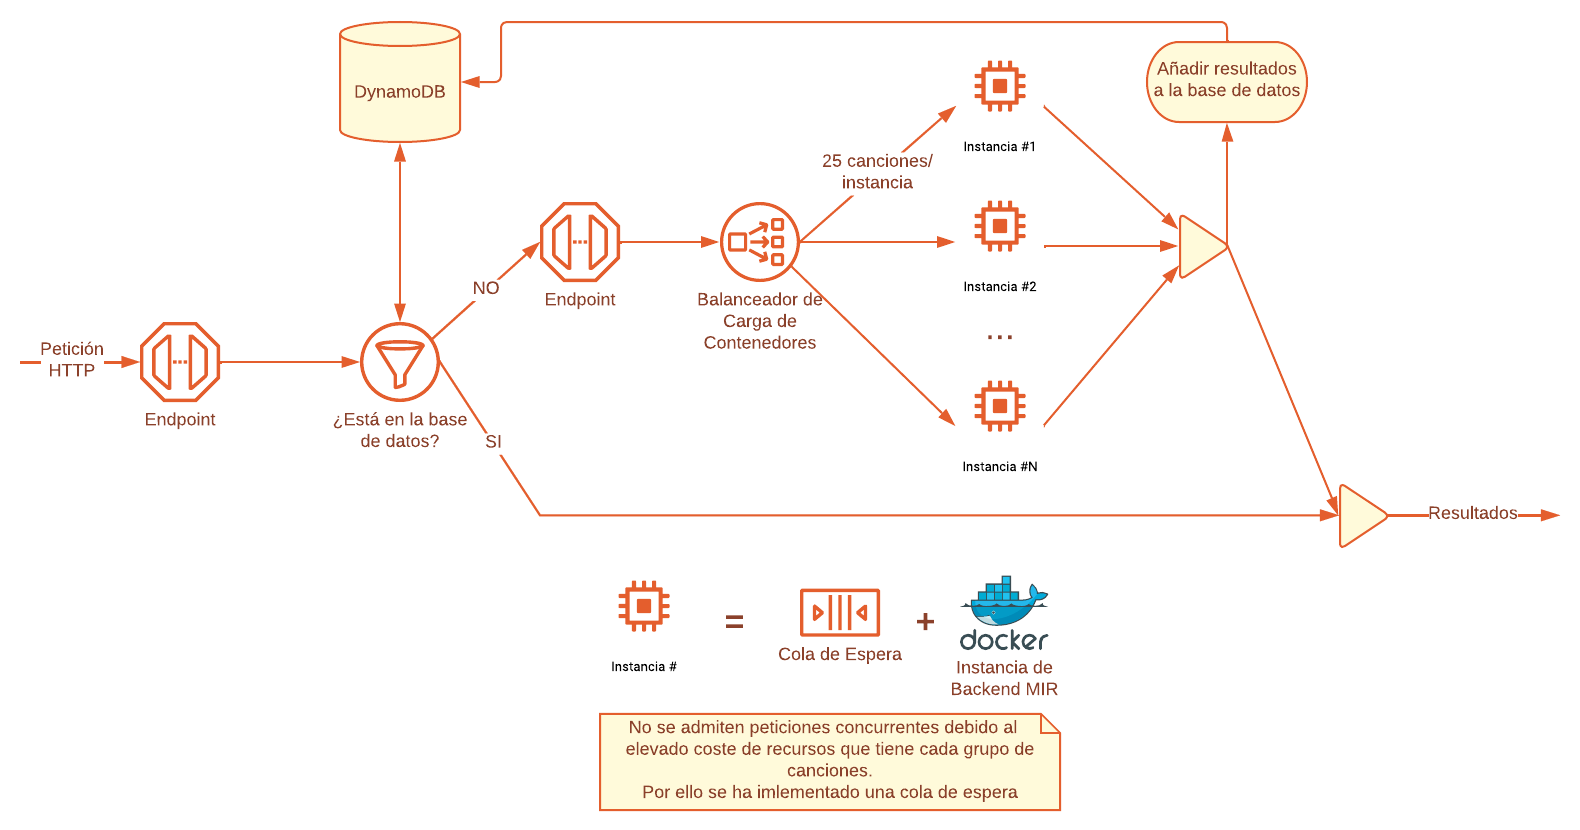
\includegraphics{img/5/ludwig_caas.png}
    \caption{Diagrama de la arquitectura CaaS del analizador.}
    \label{fig:caas_ludwig}
\end{figure}

\subsection{Etiquetas de Álbumes}\label{etiquetas-de-uxe1lbumes}

La última fuente de datos del sistema es una tabla NOSQL que almacena
las etiquetas personalizadas de los distintos usuarios.

Esta fuente de datos contiene datos dinámicos, que se pueden modificar
tanto dentro del frontend, como desde otro cliente, por lo que deben
mantenerse actualizados en todo momento.


\subsection{Caché de fuentes de
datos}\label{cachuxe9-de-fuentes-de-datos}

Algunos de estos procesos son muy lentos, como el analizador de
canciones o LastFM, y otros requieren de un gran número de peticiones,
como Spotify o LastFM, por lo que el proceso de detallar al completo una
canción o álbum puede afectar negativamente a la experiencia de usuario.

Para solventar este problema se ha implementado una caché de datos local que
permita almacenar los datos estáticos de las canciones, álbumes y
artistas en el propio navegador.
Esta caché está implementada directamente en el frontend gracias a
IndexedDB, una base de datos NOSQL presente en los estándares de W3C que
está disponible en todos los navegadores modernos.

La caché local contiene tres tablas, Track, Album y Artist, que almacenan de
forma conjunta todos los datos de cada una de las fuentes de datos.
En este caso, una canción está compuesta por un álbum y uno o más
artistas, y un álbum está compuesto por uno o más artistas.


\subsection{Fachada de Datos}\label{fachada-de-datos}

Una vez planteadas las distintas fuentes de datos y sus limitaciones,
nos encontramos con que coordinar la obtención de estos datos puede ser
una tarea muy compleja debido a los distintos estados de cada dato.

\begin{itemize}
\itemsep0em
\item
  Un dato puede estar incompleto
\item
  Un dato puede estar almacenado localmente
\item
  Una canción puede estar cacheada parcialmente (por ejemplo, puede
  estar cacheado el artista al que pertenece, pero no su álbum)
\item
  Un dato contiene datos dinámicos
\end{itemize}

Para facilitar la obtención de datos se ha implementado una fachada que
permite obtener todos los datos de manera eficiente.\\
Esta fachada permite obtener a partir de un ID o respuesta de Spotify,
un objeto completo con todos los atributos de las distintas fuentes de
datos.
Los destalles de implementación de la fachada pueden encontrarse en el Anexo C (Diseño).

\section{Aprendizaje Automático}
Para las tareas de aprendizaje automático se han utilizado redes neuronales convolucionales \ref{clasificacion_cnn}.

\subsection{Clasificador de Géneros y Subgéneros}
Para el clasificador de géneros se ha utilizado una red neuronal convolucional basada en la arquitectura EfficientNetB0 \cite{efficientnet} de Google. Se ha utilizado esta red como base debido a su capacidad de generalización para este problema.\\
En este caso, la función de activación de la capa de salida es una función $softmax()$, que normaliza la salida para que solo se active una única neurona. 

Esta red se ha entrenado con todos los géneros del Ludwig Dataset \ref{ludwig-dataset}, pero se han agrupado los géneros rock, metal y punk en un único género para reducir el número de etiquetas. Para poder diferenciar estos géneros se ha utilizado una pequeña red entrenada para diferenciar entre estos 3 géneros. 

\subsubsection{Transfer Learning}
Durante el proceso de experimentación se ha detectado una mejora en la precisión del clasificador gracias a inicializar los pesos a partir de otra red basada en EfficientNetB0. Esta red inicial ha sido entrenada con el conjunto de datos GTZAN Extended \ref{gtzan-extended}.

Una vez entrenada la red al completo con GTZAN Extended, se ha reemplazado la capa de salida de 10 neuronas por una capa de 9 neuronas, y se han vuelto a entrenar todas las capas con los nuevos datos.

\subsubsection{Clasificador de Subgéneros}
La clasificación de subgéneros es un problema de clasificación multietiqueta, ya que una canción puede tener uno o más subgéneros.

En este caso, debido a la gran cantidad de subgéneros que puede tener cada género, 
se han entrenado 11 clasificadores multietiqueta, por cada uno de los géneros principales del Ludwig Dataset \ref{ludwig-dataset}.\\
La función de activación de la capa de salida \footnote{La salida de la red tiene tantas neuronas como subgéneros.} es la función $sigmoide()$, en la que cada neurona puede tomar un valor entre 0 y 1 para indicar si la canción se corresponde a una etiqueta o no.

\subsection{Clasificador de Estados de Ánimo} \label{mood_ensemble}
La clasificación de los estados de ánimo es un problema de clasificación multietiqueta, en el que el una canción puede tener varios estados de ánimo. 

En este caso, la clasificación de los estados de ánimo se ha realizado mediante un ensemble de 7 CNNs binarias de tipo OVA \ref{one-vs-all}. Cada modelo que forma el ensemble se especializa en detectar si una canción tiene un estado de ánimo en específico o no. \\
Por último, se han juntado todos los modelos en una única red neuronal para crear el ensemble, concatenando todas las salidas binarias en un único tensor de salida. 

\subsection{Datos}

Para el entrenamiento se ha utilizado undersampling para balancear el número de datos por etiquetas.\\
\\
El clasificador de géneros ha sido entrenado con 5000 canciones por etiqueta. \\
Cada clasificador de subgéneros ha sido entrenado con 600 canciones por cada subgénero. \\
Cada clasificador de estados de ánimo ha sido entrenado con conjunto de datos en el que la mitad de los datos contienen el estado de ánimo que se desea identificar y la otra mitad no.

Estos conjuntos balanceados se han dividido en dos subconjuntos aleatorios. Por un lado, tenemos el conjunto de entrenamiento que contiene el 70\% de las canciones que vamos a utilizar, este subconjunto será utilizado para ajustar el modelo. Por otro lado, tenemos un pequeño conjunto de validación con el 30\% de las canciones restantes, que utilizaremos para evaluar la precisión final de los modelos.

Para aumentar la variedad de datos, mejorar la generalización de la red, y evitar entradas muy grandes, se han dividido todas las canciones, de 30 segundos de duración, en segmentos de 3 segundos.
Para cada uno de los segmentos se han extraído 32 MFCCs \footnote{La entrada a la red es una matriz de $32\times130$} \ref{coeficientes-cepstrales-en-las-frecuencias-de-mel}, que serán utilizados como entrada de la red. 


\subsection{Votación}
Por último, para mejorar la confianza de la predicción de cada clasificador se realiza una votación para decidir la clase final de la canción. Esta votación se realiza a partir de inferir un conjunto de fragmentos de 3s y se selecciona la etiqueta más popular de los resultados como la etiqueta final de la canción. 


\section{Sistemas de Recomendación} \label{recomend_contenido}
\subsection{Vecindad como métrica de similitud entre canciones}
Para crear un sistema de recomendación basado en contenidos se ha decidido utilizar un sistema de vecindad. Este sistema permite encontrar las canciones más cercanas o similares a una canción específica.

Para generar las instancias que van a ser comparadas, se ha decidido extraer el máximo número de datos de una canción mediante Librosa. Para resumir los resultados vectoriales o matriciales, como los MFCCs o los espectrogramas de mel \ref{coeficientes-cepstrales-en-las-frecuencias-de-mel}, se han reemplazado por su media y varianza.\\
Debido a las limitaciones del sistema, se han eliminado todos los datos cuyas operaciones de extracción tardaban más de 0.1s respeto a la media de operaciones\footnote{Algunas de las características eliminadas son los tempogramas, centroides tonales, centroides espectrales o descomposición de espectrogramas}. Y para reducir aún más el tamaño del vecindario, realizó un estudio de la correlación de los datos mediante Knime \ref{knime}. 

Los datos finales utilizados para crear el vecindario son:
\begin{enumerate}
    \item 32 medias y varianzas de los  MFCCs \ref{coeficientes-cepstrales-en-las-frecuencias-de-mel}
    \item Tempo. El tempo permite conocer como de rápido va la música.
    \item Media y varianza del tempo obtenidas de ventanas de tamaño \textit{hop\_length}.
    \item 12 medias y varianzas del cronograma. El cronograma permite conocer los tonos más importantes del espectrograma\footnote{Espectrograma en frecuencias de mel}.
    \item Media y varianza de los centroides del espectrograma
    \item Media y varianza del ancho de banda del espectrograma. Se divide el espectrograma en ventanas de tamaño \textit{hop\_length}, el ancho de banda es la porción de frecuencias más representativa en la que se representa la señal, la frecuencia central del ancho es el centroide.
    \item Media y varianza del contraste del espectrograma. Comparación entre la energía media (db) de cada ventana del espectrograma y la energía más elevada.
\end{enumerate}

Una vez creado el vecindario a partir del conjunto de datos \ref{dataset_similitud}, se normalizan los datos y se entrena un ball tree \ref{ball_tree} para poder consultar los ids de Spotify de las canciones más similares de forma eficiente.


\subsection{Sistema de Recomendación Colaborativo basado en Playlists} \label{recomend_colab}
Se ha implementado un prototipo de sistema de recomendación colaborativo basado en los contenidos de 200.000 playlists. Estas playlists de Spotify han sido recopiladas y anonimizadas por la promia compañía en \cite{million_playlist_dataset}. Para la creación y evaluación de las recomendaciones se ha utilizado la biblioteca Scikit Suprise \cite{supriselib}.\\
Este sistema de recomendación está basado en una puntuación a cada uno de los elementos de la playlist con una nota del 0 al 5, calculada a partir de la popularidad de la playlist, frecuencia de actualización, \% de canciones del mismo artista o álbum, etc.\\
Las recomendaciones iban a integrarse con la plataforma como un sistema para completar la playlist de un usuario a partir de canciones ya existentes. Se ha descartado la idea por el elevado coste de añadir nuevos datos a una matriz dispersa, ya que es necesario volver a ajustar la matriz dispersa para cada una de las peticiones de recomendación.\\
Por otro lado se han intentado obtener las recomendaciones más cercanas a a otra mediante la implementación de un algoritmo de vecindad de Surprise, pero debido a que esta implementación no usa matrices dispersas, el consumo de memoria necesario para obtener las canciones más cercanas es demasiado alto, por lo que la implementación de esta característica no es viable a nivel de recursos.


\section{Arquitectura Contenedores}

Se ha dividido la arquitectura en cuatro servicios, \textbf{frontend}, \textbf{servidor principal o servidor NextJS}, \textbf{base de datos} y \textbf{servidor recuperación de información musical}\footnote{También referido como Backend MIR o Backend Ludwig}. 

Estos cuatro servicios se han agrupado en tres contenedores Docker\ref{docker} distintos interconectados, como muestra la figura \ref{fig:arquitectura_contenedores}.\\
El servicio puede levantarse en una sola máquina gracias a Docker Compose, se recomienda consultar el manual de instalación y despliegue en los anexos. 

\subsection{Contenedor NextJS}
El contenedor NextJS contiene el frontend y el servidor principal, ya que ambos se ejecutan sobre un mismo servidor de NextJS. 

El servicio de frontend se encarga del renderizado parcial en el servidor de las distintas páginas y componentes web, así como de la distribución de las páginas y ficheros estáticos.

El servicio de servidor NextJS es una pequeña API REST que se encarga de gestionar operaciones con datos sensibles, como la autenticación del usuario, eliminación de la cuenta o la gestión de tokenes JWT \ref{jwt}. Por otro lado, para reducir el acoplamiento del sistema, se ha decidido que este servicio sea el único servicio con acceso a la base de datos.\\
Esta API Rest ha sido configurada para permitir la política de seguridad CORS\footnote{Intercambio de Recursos de Origen Cruzado, el frontend puede acceder a recursos del servidor sin necesidad de compartir dominio.}, por lo que el frontend y el servidor pueden desplegarse por separado.


\subsection{Contenedor DynamoDB}
El contenedor DynamoDB contiene una instancia de DynamoDB Local \ref{dynamodb-y-dynamoose}, la única base de datos del sistema\footnote{Sin tener en cuenta la caché del frontend con DexieDB}. 
Este contenedor no está pensado para ser desplegado a producción, ya que una de las principales ventajas de DynamoDB es que es una base de datos administrada que se despliega en un cluster para mejorar su rendimiento. Para más información se recomienda consultar el apartado de despliegue \ref{deployment}.

\subsection{Contenedor Ludwig MIR}
El contenedor Ludwig MIR contiene una API de python que se encarga del preprocesamiento y análisis de canciones en cualquier formato de audio\footnote{Gracias a FFMPEG}.\\
La política de seguridad de este contenedor obliga a todas las peticiones a portar un token de seguridad en la cabecera  \code{Authentication}. Este token es un código secreto estático que debe ser compartido entre todos los servicios que desean interactuar con el contenedor. En este caso, únicamente el contenedor NextJS tiene acceso a este código, por lo que actúa como intermediario.\\
Debido al elevado coste de descargar, preprocesar y analizar canciones, se ha planteado el uso de una pequeña caché que almacene los resultados en DynamoDB. La lógica de esta caché está gestionada por el servidor de NextJS.


\section{Pruebas e Integración Continua}
\subsection{Pruebas Unitarias}
Se han realizado pruebas unitarias sobre los componentes de la capa de presentación, como los clientes REST, y clases y funciones auxiliares. 
Debido a la dificultad de renderizar componentes fuera de un navegador, ya que no todas las funcionalidades se pueden ejecutar fuera de un navegador sin el uso de mocks\footnote{Clases o funciones esqueleto que contienen todas las operaciones de la clase real, no todas las bibliotecas incluyen mocks.}, se ha descartado realizar pruebas unitarias exhaustivas en la capa de la Vista.\\
Estas pruebas han sido realizadas mediante la biblioteca JEST \ref{jest}

\subsection{Pruebas Punto a Punto}
Se han realizado pruebas automáticas y de sistema a la interfaz web, así como a los distintos endpoints de las APIS mediante Cypress \ref{cypress}. Estas pruebas se realizan directamente sobre la web desplegada.
Los endpoints han sido implementados siguiendo la metodología TDD \ref{test_driven_dev}.

\subsection{Integración Continua}
Se ha programado mediante Github Actions \ref{github-actions} la ejecución de las distintas pruebas tras cada operación de push y merge al repositorio. Estas acciones permiten generar reportes sobre el estado del proyecto, y detectar los fallos en el momento en el que se actualiza el proyecto. 

\section{Despliegue Continuo}\label{deployment}
\subsection{Google Cloud Run}
Se han desplegado en contenedores de \ref{google-cloud-run} los servicios NextJS Backend y Ludwig Backend.
Estos contenedores se generan y despliegan automáticamente\footnote{Gracias a Google Container Registry, esta operación se puede delegar a Github Actions} tras cada push que modifique los backends en el proyecto.

El contenedor NextJS se ha alojado en máquinas con apenas 256MB de RAM y un núcleo, ya que este contenedor apenas realiza operaciones con un elevado coste de recursos. \\
Este contenedor tiene libertad para escalar automáticamente.

El contenedor Ludwig Backend se ha desplegado en máquinas con 2GB de RAM y un núcleo. Estos contenedores están pensados para procesar hasta 25 canciones al mismo tiempo, por lo que necesitan un mayor número de recursos para inferir con todas la redes neuronales.\\
Para reducir el consumo de recursos, se han cuantizado \ref{cuantizacion-de-redes-neuronales} los modelos a UINT8, reduciendo el consumo de memoria un contenedor de 6.8GB a menos de 2GB de RAM.
Los consumos de memoria son tan elevados debido a que trabajamos con bloques de canciones para acelerar la inferencia.\\ 

Para acelerar el proceso de inferencia de un gran grupo de canciones, el orquestador está configurado para levantar el máximo número de contenedores en vez de encolar las peticiones de inferencia en grupos de 25 canciones. Se ha configurado un límite de 350 contenedores simultáneos antes de que el sistema empiece a encolar las peticiones de inferencia.

\subsection{Vercel}\label{vercel_deployment}
El propio frontend de NextJS es transpilado, optimizado y desplegado por la plataforma Vercel \ref{vercel-plataforma}.
Vercel, a diferencia de Google Cloud Run, no admite contenedores personalizados, pero está diseñada para optimizar, desplegar y escalar proyectos de NextJS.\\
Se ha configurado Vercel para realizar un despliegue automáticamente por cada push y pull request que se realice en el repositorio del proyecto\footnote{Al igual que GCP, se puede automatizar mediante Github Actions}. 

El servidor web de NextJS no se ha desplegado junto a su frontend por las limitaciones del plan gratuito de Vercel, ya que una petición al servidor no puede durar más de 10s, un tiempo muy bajo para que Ludwig pueda inferir los bloques de 25 canciones. 

\subsection{Amazon Web Services}
En este caso se ha utilizado el servicio DynamoDB \ref{dynamodb-y-dynamoose} para la base de datos. Este servicio permite controlar y escalar la base de datos en al menos dos clusters, dividiendo los datos a patir del hash de los índices. 
Las tablas son gestionadas automáticamente gracias a Dynamoose, por lo que todas las actualizaciones se propagan a la base de datos de AWS. 


